\section{Species}
\DndDropCapLine{T}{}he custom or adapted species section in this grimoire serves to elaborate on the history of the world and its denizens. They are \textbf{Seraphs, Elves, Drakeborn, Orqs, Dwerfens , Golyaths, Halflings, Tieflings,} and of course \textbf{Humans}.

\begin{figure}[H]
    \centering
    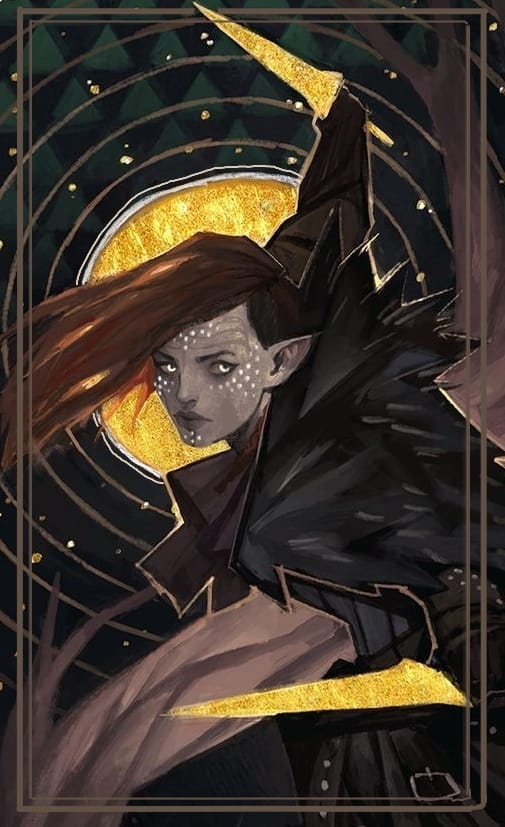
\includegraphics[width=0.58\linewidth]{Images/drow_assassin.jpeg}
    \label{fig:placeholder}
\end{figure}
\begingroup
\DndSetThemeColor[PhbMauve]
\begin{DndSidebar}{The Knives in the dark...}
\textit{}
\end{DndSidebar}
\endgroup

\subsection{Elves}
Descendent from the \textbf{primordial elves} that first inhabited the known world, they are the main humanoids ruling over their respective kingdoms in the far and not so far corners of this campaign. With \textit{ears like blades and varying adaptations to their namesake environs}, elves are the most versatile and abundant race second only to \textbf{humans}.

\subsubsection{High Elf}
\textit{Gladiatorial and Greco-Roman culturalists of decadent design}, \textbf{high elves} rule the \textbf{largest kingdom of Romulon}, the political and religious nexus of the known world. With golden-metallic skin and thick fair hair, some argue they are the most beautiful of the modern elves.

\subsubsection{Dark Elf \textit{(Drow)}}
The deep elves of the\textbf{ underdark} differ from their fair-skinned cousins only in hue, \textit{with brass and bronze skin and pale grey or dirty blonde hair, these elves boast bioluminescent marks that match their red and purple glowing eyes} made to see the \textbf{underdark's} darkest corners. Predominantly from the city \textbf{near the undersea - Latibulus}.

\subsubsection{Wood Elf \textit{(Dryad)}}
These primal Elves of the wooded variety embody nature like none other, bound by the \textbf{verdant oath}, these elves may not harm nature by any means. \textit{With horns and pale green, marked skin, these elves have lost their metallic glamour in favour of pragmatic features to hunt}. Their main settlements are sprinkled wherever there are forests and jungles, but the biggest by far is \textbf{Kaer Holte}, better known as the \textbf{"Hollow Keep"} within the \textbf{Phenozimal Jungle}.

\subsubsection{Snow Elf}`
An offshoot of the wood elves, \textbf{snow elves} were an \textit{advanced civilization of astrologers and scholars of the heavens}; \textbf{occult interference rendered the race lost to time}. \textit{With pearlescent hair, metallic silver skin, claws and dark eyes like the night sky, they branched when the wood elves were still nascent to the primal elves}. The lost citadel of \textbf{Tír Astrada} was the home the original royal line, sadly it is a plundered mess of ruins in modern times.

\subsection{Elf Traits}
The base Elven traits and characteristics are the same as in the \textit{2024 PHB}.

The subspecies of Elf you are determines the evolutionary magicks you possess. The spells available to you manifest at levels 1, 3 and 5 as you mature in power.

These are the same as in the \textit{2024 PHB}, for \textbf{snow elves} you learn the \textit{light cantrip} and gain \textit{resistance to frost damage} at level 1, you additionally learn \textit{ice knife} and \textit{mirror image} at levels 3 and 5 respectively. 

The race is \textit{only playable at the discretion of the game master} as they are \textbf{presumed extinct}.

\begin{DndReadAloud}
   The Elves were the original race of beings on this world, it is only with the arrival of the humans in a cosmic event that the other exotic species arose from their enigmatic roots.
\end{DndReadAloud}

\subsection{Dwerfen}
The "Dwarves" or the more technically correct term in the current world is that of the \textbf{Dwerfen}. \textit{Reclusive and Greedy engineers of brass marvels}, these Persian inspired denizens of the \textbf{Deep Roads} live much \textit{farther underground} than the \textbf{Drow} and almost never surface unless for \textit{political or trade reasons}. \textit{Elf-like in appearance, this species bears no ties to the Elves, instead originating from far below the world's crust}.

Generations of proximity to lyrium ore veins have made dwarves naturally resistant, though not completely immune, to its effects. Even their resistance is only skin deep, as direct exposure of raw lyrium to open cuts, inhalation, or contact through the eyes or mouth leaves them vulnerable to side effects. The side effects are usually non-lethal so long as the amount of lyrium and frequency of invasive exposure is minimal. Surface dwarves lose this resistance over time.

\subsection{Orqs}
Wood Elves \textit{cursed to savagery in opposition to their intrinsic harmony with nature}, \textbf{Orqs} resemble their Elven ancestors faintly, having traded their \textit{antler horns for wolven canines and ridged faces} and a hunger for conquest.\textbf{ The Pariah-Folk} are found in \textit{dessicated forests and torn-down jungles}, used to fuel their engines of war.

\subsection{Golyaths}
Towering over most folk, \textbf{golyaths} are distant \textit{de-
scendants
of
giants, a primordial demi-deitic race of beings that with time became the landscape we now find ourselves traversing. Though mostly extinct, some giants can be found in the extrema of the worlds elements}. Each \textbf{golyath} bears the favours
of
the first
giants. Favours that
manifest in various
supernatural boons, including the ability to quickly
grow and temporarily approach the height
of
golyaths' gigantic kin.
\textit{Golyaths have physical characteristics that are
reminiscent
of
the giants in their family lines}. For
example, some \textbf{golyaths} look like stone giants, while
others resemble fire giants.

\subsection{Drakeborn}
The \textbf{Drakeborn} are an \textit{oviparous race of scaled humanoids}. Their \textit{draconic features mirror their culture's archaic medieval dogma}, although curiously \textbf{hive-minded}, the there \textit{is room for individual ambition and emotion}. Whether humans were \textit{cursed or gifted with the essence of dragons} is unknown, as is most of their culture. They are themed for the types of dragons and vary in how lizardlike they appear. \textbf{They use the abilities of the Forgotten Realms' Dragonborn}.

\begin{figure}[H]
    \centering
    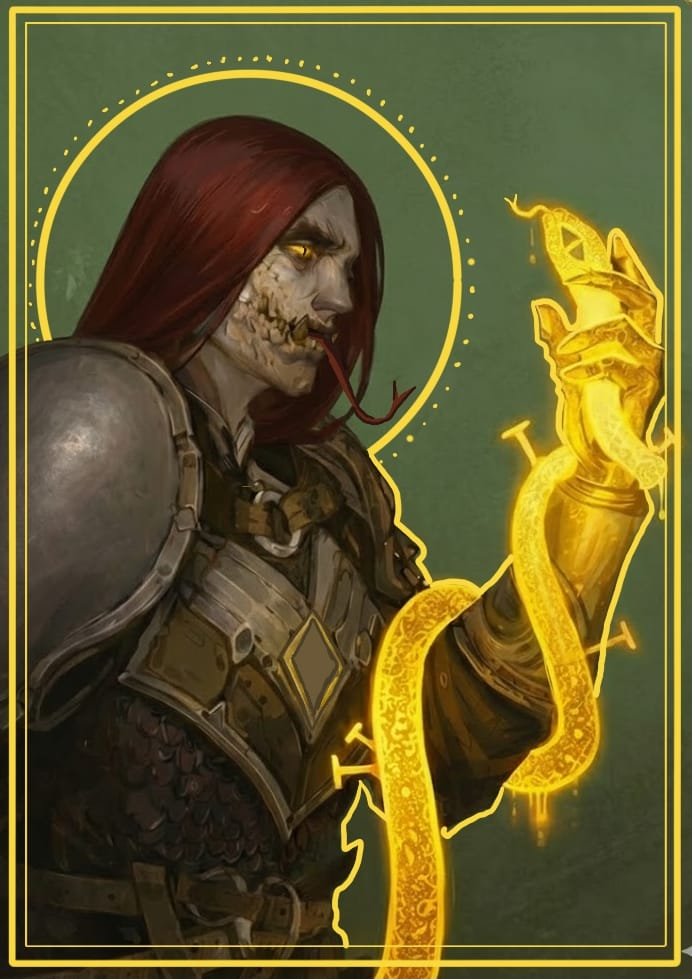
\includegraphics[width=0.64\linewidth]{Images/argonian.jpeg}
    \label{fig:placeholder}
\end{figure}

\begingroup
\DndSetThemeColor[PhbMauve]
\begin{DndSidebar}{Scaled and Cold-blooded}
\textit{Hivemind-driven Scaled Ones, known as the Drakeborn.}
\end{DndSidebar}
\endgroup

\subsection{Halflings}
Small critters from the \textbf{Everglade}, \textit{a permanently spring/autumnal meadowland perfect for farming and respite.} Generally kind and unambitious.

Anyone
who has spent
time around \textbf{halflings}, particularly halfling
adventurers
, has likely witnessed
the \textit{storied "luck
of
the halflings"} in action. When a
halfling is in
mortal danger
, \textit{an unseen force seems
to intervene on the halfling's behalf}.

\subsection{Humans}
\textbf{Humans }are as
\textit{varied as they are numerous}, and they endeavor to
achieve as much as they can in the years they are
given.\textit{ Their ambition and resourcefulness are commended, respected, and feared by all races, though the individual human is more a blank canvas than a creature of great power.}

\subsection{Seraphs}
\textbf{Seraphs} \textit{are mortals
who carry a greater spark of the outer deities within their
souls}. Whether descended from an angelic being or
infused with celestial power, they can \textit{arc that essence outward
to bring light, healing, and heavenly fury. Additionally they exhibit supernatural traits such as resistances and enhanced senses}.
However you are inclined to believe, these divine traits often \textit{manifest in biblically frightening ways} as supposed to the usual winged elven appearance.

\begin{figure}[H]
    \centering
    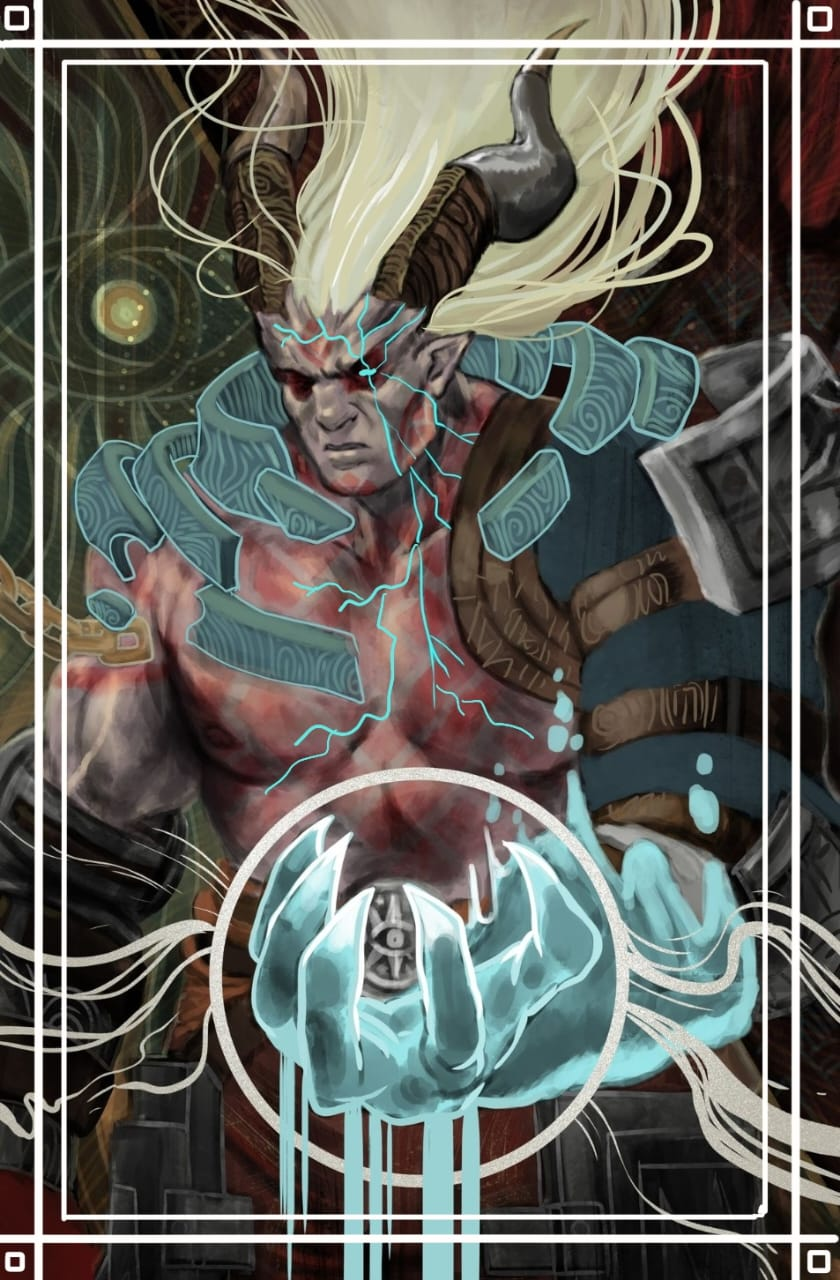
\includegraphics[width=0.64\linewidth]{Images/saarebas.jpeg}
    \label{fig:placeholder}
\end{figure}

\begingroup
\DndSetThemeColor[PhbMauve]
\begin{DndSidebar}{Saarebas or "Dangerous One"}
\textit{The Abyssal Tieflings borne of \textbf{Dremoric influence} have unified under a banner of \textbf{strict religion} in opposition to their evil origin.}
\end{DndSidebar}
\endgroup


\subsection{Tieflings}
Lineages cursed through \textit{occult dealings or less than savoury unions}, \textbf{Tieflings} bear resemblance to christian depictions of demons, though they vary in origin and diverge to appearances alien or common. The source of a lineage determines the appearance and most members of these ethnicities, shunned by the other cultures, have \textit{gathered into kingdoms and formed unique cultures of their own}.

\subsubsection{Infernal}
\textbf{Infernal Tieflings}, shunned by all god-fearing people, are \textit{Luciferian individuals in appearance alone}, for they are \textbf{not intrinsically evil at all}, merely an unfortunate byprodcut of their circumstance. Some adhere to the stereotype, whether it be nature or nurture, and reinforce the stigma binded to them. \textit{Horns, spines, tails, golden eyes and a faint odour of sulphur are common physical features} to these creatures that trace their ancestry to \textbf{Devils} of the \textbf{Nine-Hells}. These tieflings classify as \textbf{\textit{fiends}}.


\subsubsection{Abyssal}
The beastly, muscular tieflings of \textbf{Dremoric} origin have collected to a \textit{large empire of lawful strictness} know as the \textbf{Vashoth or "Grey Ones"} symbolising their \textit{neutral choice of alignment}, \textit{rejecting the chaotic evil nature of their} \textbf{Dremoric} \textbf{ancestry of }\textbf{Oblivion}. The females appear \textit{more alienlike} and exhibit \textit{extra eyes and an improved perception}. These tieflings classify as\textit{\textbf{ fiends}}.

There are \textbf{no Abyssal Tiefling wizards}\textit{ since magic is outlawed}, however those \textbf{born with magical powers are shackled} and \textit{forced to imbibe}\textbf{ Lyrium}, \textit{a bluish crystal substance that empowers a spell to no longer require any components and able to be cast with instinct alone}. These abominations are known as \textbf{Saarebas}.

\begin{DndReadAloud}
   The Elves were the original race of beings on this world, it is only with the arrival of the humans in a cosmic event that the other exotic species arose from their enigmatic roots.
\end{DndReadAloud}

\subsubsection{Cthonic}
"Gravely" in appearance and tragically misunderstood, the \textbf{Chthonic tieflings} are the\textit{ most terrifying in appearance, with horns that seemingly grow out the eye-sockets}. They are \textbf{physically blind}, but are able to sense their surroundings magically and have effective \textbf{blindsight to a range of 15 m} around them. Just like their \textbf{infernal and abyssal cousins}, \textit{they contain no malignant nature from birth and are generally the kindest of the tieflings despite their melancholic circumstance}. \textit{Favouring jewelry and fancy clothes to appear less monstrous}, these tieflings often own large businesses with less horrific looking races performing trade for public relations. These tieflings classify as \textbf{\textit{aberrations}}.

\begin{figure}[H]
    \centering
    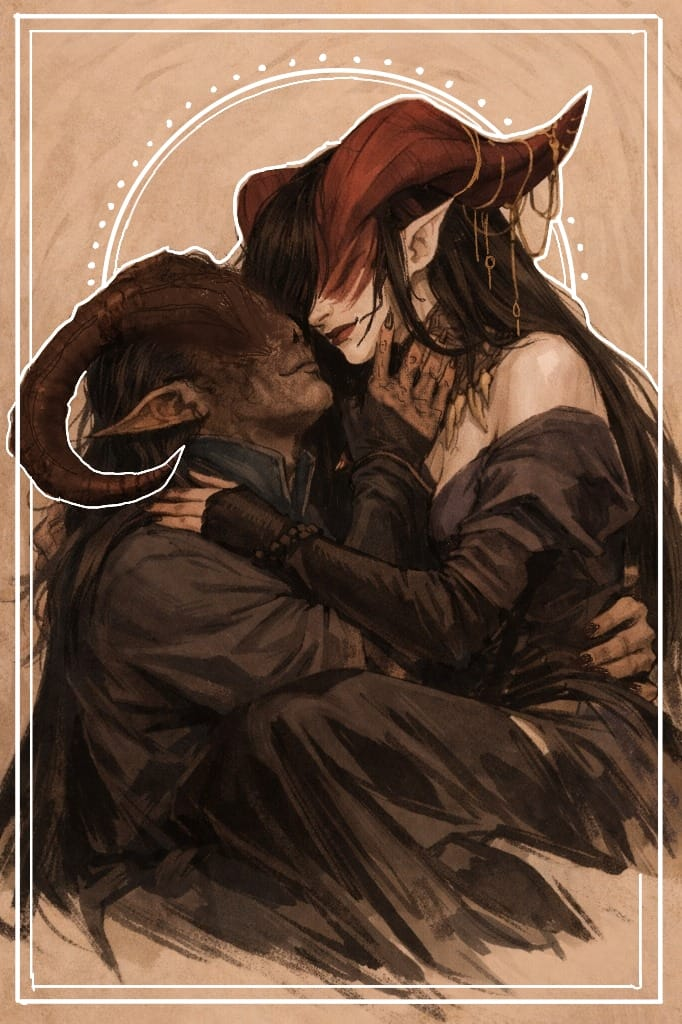
\includegraphics[width=0.64\linewidth]{Images/cthonic.jpeg}
    \label{fig:placeholder}
\end{figure}

\begingroup
\DndSetThemeColor[PhbMauve]
\begin{DndSidebar}{A face that only a mother could Love}
\textit{The \textbf{Cthonic Tieflings} are the least common and most misunderstood, but to understand another deeply is to see them, to Love.}
\end{DndSidebar}
\endgroup
